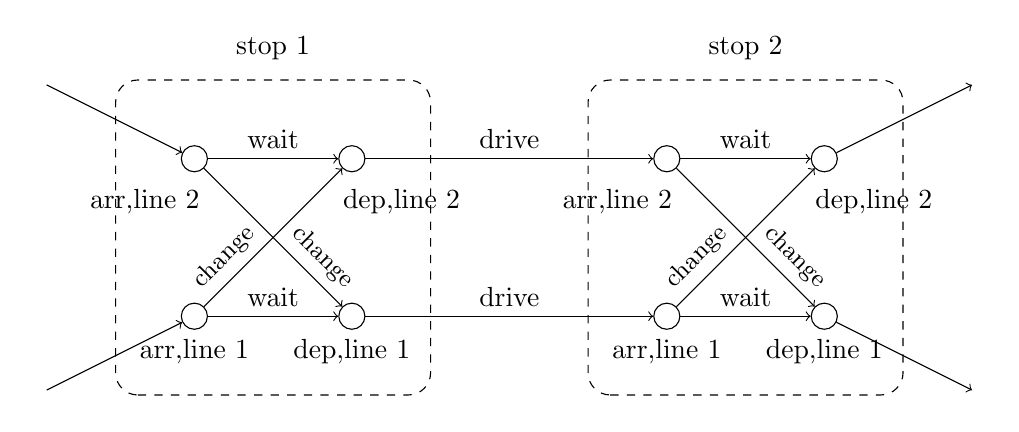
\begin{tikzpicture}[scale=2]
    % \node {Hei moi!};
    \tikzstyle{node}=[circle,draw]
    
    
    % \foreach \x in {0,1}
    %     \foreach \y in {0,1}
    %         \node (s1-\x-\y) at (\x, \y) [node,label=] {};
    % \foreach \y in {0, 1}
    %     \node (s1-ext-\y) at (-1, \y) {};
    
    \node (0-0) at (0, 0) [node, label={below:arr,line 1}]{};
    \node (1-0) at (1, 0) [node, label={below:dep,line 1}]{};
    \node (3-0) at (3, 0) [node, label={below:arr,line 1}]{};
    \node (4-0) at (4, 0) [node, label={below:dep,line 1}]{};
    \node (ext1-0) at (-1, -0.5) {};
    \node (ext2-0) at (5, -0.5) {};
    
    
    \node (0-1) at (0, 1) [node, label={[shift={(-0.63cm,-1cm)}]arr,line 2}]{};
    \node (1-1) at (1, 1) [node, label={[shift={(+0.63cm,-1cm)}]dep,line 2}]{};
    \node (3-1) at (3, 1) [node, label={[shift={(-0.63cm,-1cm)}]arr,line 2}]{};
    \node (4-1) at (4, 1) [node, label={[shift={(+0.63cm,-1cm)}]dep,line 2}]{};
    \node (ext1-1) at (-1, 1.5) {};
    \node (ext2-1) at (5, 1.5) {};
    
    
    % \foreach \x in {3,4}
    %     \foreach \y in {0,1}
    %         \node (s2-\x-\y) at (\x, \y) [node] {};
    % \foreach \y in {0, 1}
    %     \node (s2-ext-\y) at (5, \y) {};
    
    \draw [->] (ext1-0) to (0-0);
    \draw [->] (0-0) to node [above] {wait} (1-0);
    \draw [->] (1-0) to node [above] {drive} (3-0);
    \draw [->] (3-0) to node [above] {wait} (4-0);
    \draw [->] (4-0) to (ext2-0);
    
    \draw [<-] (ext2-1) to (4-1);
    \draw [<-] (4-1) to node [above] {wait} (3-1);
    \draw [<-] (3-1) to node [above] {drive} (1-1);
    \draw [<-] (1-1) to node [above] {wait} (0-1);
    \draw [<-] (0-1) to (ext1-1);

    \draw [->] (0-1) to node [near end, above, sloped] {\small change} (1-0);
    \draw [->] (0-0) to node [near start, above, sloped] {\small change} (1-1);

    \draw [->] (3-1) to node [near end, above, sloped] {\small change} (4-0);
    \draw [->] (3-0) to node [near start, above, sloped] {\small change} (4-1);
    
    \draw [rounded corners=8, dashed] (-0.5, -0.5) -- (1.5, -0.5)
        -- (1.5, 1.5) -- (-0.5, 1.5) -- cycle;
    
    \draw [rounded corners=8, dashed, xshift=3cm] (-0.5, -0.5) -- (1.5, -0.5)
        -- (1.5, 1.5) -- (-0.5, 1.5) -- cycle;
    
    
    \node at (0.5, 1.7) {stop 1};
    \node at (3.5, 1.7) {stop 2};
    
\end{tikzpicture}